\section{A Kinematic Model for HSA Rods}\label{sec:hsamodel:hsa_rod_kinematics}
In this section, we aim to derive a forward kinematic model that can be used to describe the shape of a single \gls{HSA} rod with a minimum amount of parameters. More specifically, we want to describe the transformation from the base frame $\{ S_{\mathcal{B}} \}$ to a local frame $\{ S_s \}$, a coordinate $s \in (0, \Bar{L}]$, which is a function of the soft robot's configuration $q$. This coordinate lies on the backbone of a \gls{HSA} rod of printed (i.e., initial) length $\Bar{L}$.

\subsection{Selective Piecewise Constant Strain (SPCS) Kinematics}\label{sub:hsamodel:hsa_rod_kinematics:spcs_kinematics}
For this purpose, we combine the existing kinematic models \gls{CS} and \gls{PCS}~\citep{renda2018discrete} to selectively keep specific strains constant along the entire length of the robot or vary them piece-wise among the segments.
%Opposite to existing kinematic models based on \gls{CC}~\citep{garg2022kinematic}, our kinematic description strives to model the twist of the \gls{HSA} rod.
This parametrization can be combined with the results in Sec.~\ref{sec:hsamodel:hsa_robot_simulation} to generate a compact dynamic model for the movement of HSA robots in 3D space.
\begin{figure}[htb]
    \centering
    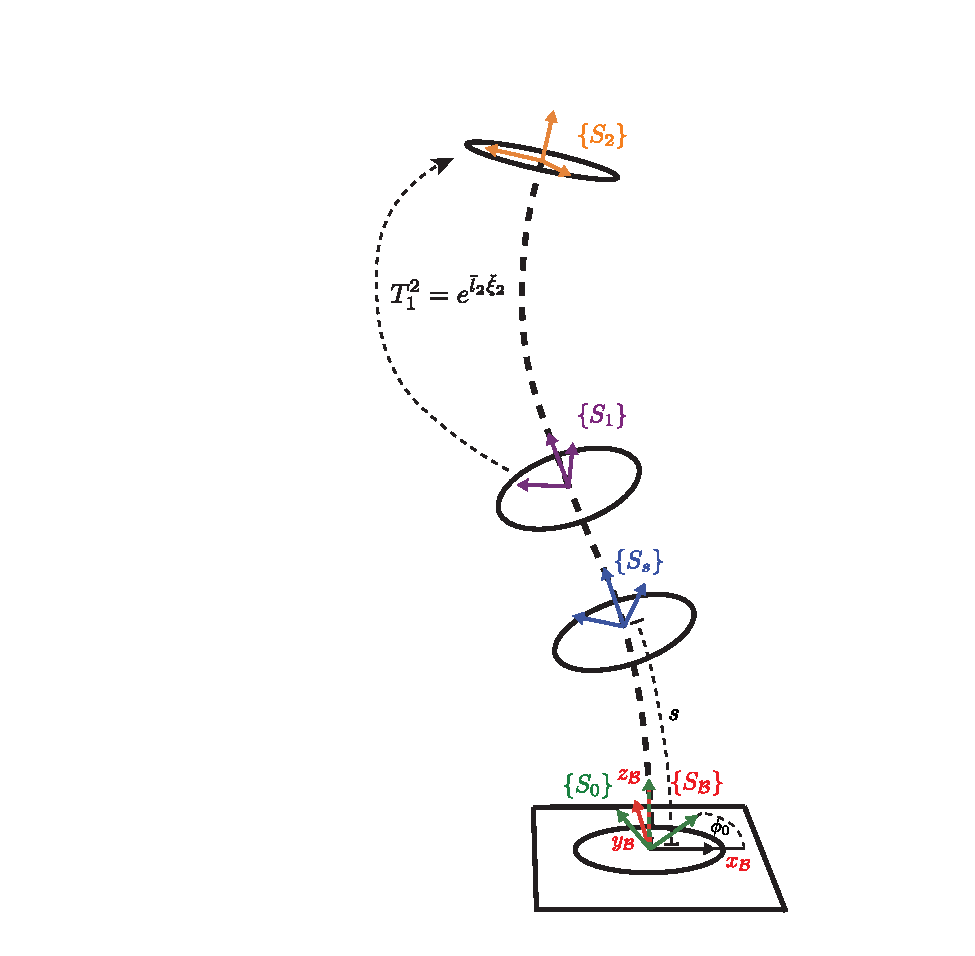
\includegraphics[width=0.25\columnwidth]{hsamodel/figures/kinematics/twisting_kinematics_v2_cropped.pdf}
    \caption{Visualization of the proposed \gls{SPCS} kinematic model for the case of $n_\mathrm{S} = 2$ segments: The forward kinematics describe a transformation from the base frame $\{ S_{\mathcal{B}} \}$ to the local frame $\{ S_s \}$ at the coordinate $s \in [0, \bar{L}]$ and consist of a) a rotation around the $z_{\mathcal{B}}$-axis of the base frame by angle $\phi_0$, b) an exponential map $e^{(s-\bar{L}_i) \, \check{\xi}_i}$ for the transformation from the proximal end of the $i$th segment to the local frame of the coordinate $s$. % The strain $\xi_i$ consists of a rest strain $\hat{xi}$, a strain $\xi_{\mathrm{CS}}$ constant along the entire rod, and finally a strain component specific to the $i$th segment $\xi_{\mathrm{PCS},i}$.
    }
    \label{fig:hsamodel:hsa_kinematics}
\end{figure}

First, we define that 
\begin{equation}
    \xi(q,s) = \begin{pmatrix} \kappa_x & \kappa_y & \kappa_z & \sigma_x & \sigma_y & \sigma_z \end{pmatrix}^\top \in \mathbb{R}^6
\end{equation}
represents the three rotational and three linear strains present in a rod~\citep{renda2018discrete}. Subsequently, propose the following configuration vector for an \gls{HSA}
\begin{equation}
    q = \begin{pmatrix}
        \phi_0 & q_\mathrm{CS}^\top & q_{\mathrm{PCS},1}^\top & \cdots & q_{\mathrm{PCS},i}^\top & \cdots & q_{\mathrm{PCS},n_\mathrm{S}}^\top
    \end{pmatrix}^\top% \in \mathbb{R}^{1 + n_{q,\mathrm{CS}} + n_\mathrm{S} \: n_{q,\mathrm{PCS}}},
\end{equation}
where $\phi_0 \in \mathbb{R}$ is the twist angle at the base and allows for the rotation of the motor actuating the \gls{HSA} rod. $q_\mathrm{CS} \in \mathbb{R}^{n_{q,\mathrm{CS}}}$ is a strain component constant along the entire rod, and $q_{\mathrm{PCS},i} \in \mathbb{R}^{n_{q,\mathrm{PCS}}}, i \in \{1, \dots, n_\mathrm{PCS}\}$ is the configuration of each \gls{PCS} segment. The $i$th segment has a initial length of $\bar{l}_i$ with its tip at the coordinate $\bar{L}_i$
%
The strain in the $i$th segment is then the sum of the rest strain $\xi^0 = \begin{pmatrix} 0 & 0 & 0 & 0 & 0 & 1\end{pmatrix}^\top$, $\xi_\mathrm{CS}$, and $\xi_{\mathrm{PCS},i}$:
\begin{equation}
    \xi_i = \xi^0 + \Phi_\mathrm{CS} \: q_\mathrm{CS} + \Phi_{\mathrm{PCS},i} \: q_{\mathrm{PCS},i}, \quad i \in \{1,\dots, n_\mathrm{S}\}.
\end{equation}
Analogue to the concept introduced in \citep{renda2020geometric}, $\Phi_\mathrm{CS} \in \mathbb{R}^{6 \times n_{q,\mathrm{CS}}}$, $\Phi_\mathrm{PCS} \in \mathbb{R}^{6 \times n_{q,\mathrm{PCS}}}$ are the strain bases of $q_\mathrm{CS}$ and $q_\mathrm{PCS}$ respectively.

In this chapter, we specifically investigate a setting where the twist \& stretch strains are constant across the entire rod and the bend \& shear strains vary for each segment.
Accordingly, we choose $q_\mathrm{CS} = \begin{pmatrix} \kappa_z & \sigma_z \end{pmatrix}^\top$ and $q_{\mathrm{PCS},i} = \begin{pmatrix} \kappa_{x,i} & \kappa_{y,i} & \sigma_{x,i} & \sigma_{y,i} \end{pmatrix}^\top$.
Then, the corresponding strain bases are determined to be
\begin{equation}
\begin{split}
    \Phi_\mathrm{CS} = \begin{bmatrix}
        0 & 0 & 1 & 0 & 0 & 0\\
        0 & 0 & 0 & 0 & 0 & 1\\
    \end{bmatrix}^\top \in \mathbb{R}^{6 \times 2},\\
    \Phi_{\mathrm{PCS},i} = \begin{bmatrix}
        1 & 0 & 0 & 0 & 0 & 0\\
        0 & 1 & 0 & 0 & 0 & 0\\
        0 & 0 & 0 & 1 & 0 & 0\\
        0 & 0 & 0 & 0 & 1 & 0\\
    \end{bmatrix}^\top \in \mathbb{R}^{6 \times 4}.
\end{split}
\end{equation}

Next, we find homogeneous forward kinematic mappings for the given configuration and strains.
As the twist angle $\phi_0$ demands a rotation around the local $z_{\mathcal{B}}$-axis of the base frame, the matrix $R_{\mathcal{B}}^0(\phi_0) \in SO(3)$ contains the rotation from the base frame $\{ S_{\mathcal{B}} \}$ to the proximal end of the rod denoted as frame $\{ S_{0} \}$.
For a point $s$ on the $i$th segment with constant strain $\xi_i$, the transformation matrix from the segment's proximal frame $\{ S_{i-1} \}$ to the local frame at coordinate $s$ is given by the exponential map $e: \mathfrak{se}(3) \mapsto SE(3)$~\citep{renda2018discrete}
\begin{equation}
\begin{split}
    e^{(s-\bar{L}_{i-1}) \check{\xi}_i} =& I_4 + (s-\bar{L}_{i-1}) \, \check{\xi}_i + \left ( 1 - \cos((s-\bar{L}_{i-1}) \, \theta_i) \right )\\ 
    &\frac{\check{\xi}_i^2}{\theta_i^2} + \left ( (s-\bar{L}_{i-1}) \, \theta_i - \sin((s-\bar{L}_{i-1}) \theta_i) \right ) \frac{\check{\xi}_i^3}{\theta_i^3}.
\end{split}
\end{equation}
where $\check{\xi}_i \in \mathfrak{se}(3)$ is the strain twist vector and $\theta_i = \sqrt{\kappa_{x,i}^2 + \kappa_{y,i}^2 + \kappa_{z,i}^2}$ is the magnitude of the rotational strain.
Therefore, the fully assembled transformation $T_{\mathcal{B}}^i(q)$ from the base frame $\{ S_{\mathcal{B}} \}$ to the tip frame of the $i$th segment can be expressed as
\begin{equation}
    T_{\mathcal{B}}^i(q) = T_{\mathcal{B}}^0(\phi_0) \: \Pi_{j=1}^{i} \: e^{\bar{l}_{j} \check{\xi}_{j}}(q) \in SE(3).
\end{equation}

% \begingroup
% \setlength{\tabcolsep}{3pt} % Default value: 6pt
% \begin{table}
% \centering
% \caption{Verification of kinematic model in simulation.}
% \begin{tabular}{l c c ccc}\toprule
% \textbf{Dataset} & $e_t$ [mm] & $e_\mathrm{quat}$ [-] & $e_\mathrm{eul,x}$ [rad] & $e_\mathrm{eul,y}$ [rad] & $e_\mathrm{eul,z}$ [rad]\\
% \midrule
% Elongation & \SI{0.042}{mm} & $0.00027$ & $5.6\mathrm{e}{-9}$ \si{rad} & $1.9\mathrm{e}{-8}$ \si{rad} & $1.7\mathrm{e}{-6}$ \si{rad}\\
% \bottomrule
% \end{tabular}
% \label{tab:hsamodel:kinematic_results_simulation}
% \end{table}
% \endgroup

\begin{figure}[t]
    \centering
    \subfigure{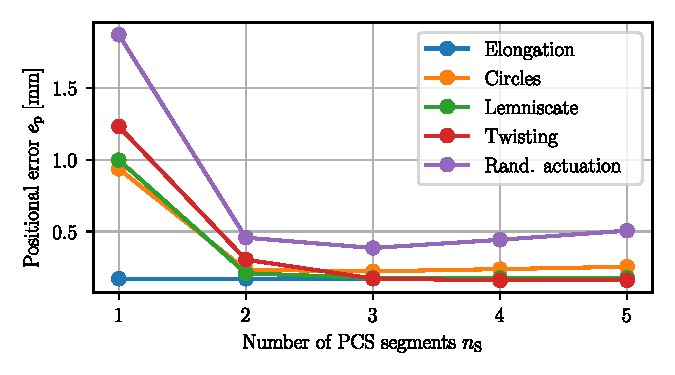
\includegraphics[width=0.49\columnwidth]{hsamodel/figures/simulation_plots/Kinematic_position_error_vs._number_of_PCS_segments_v3_cropped.pdf}}
    \subfigure{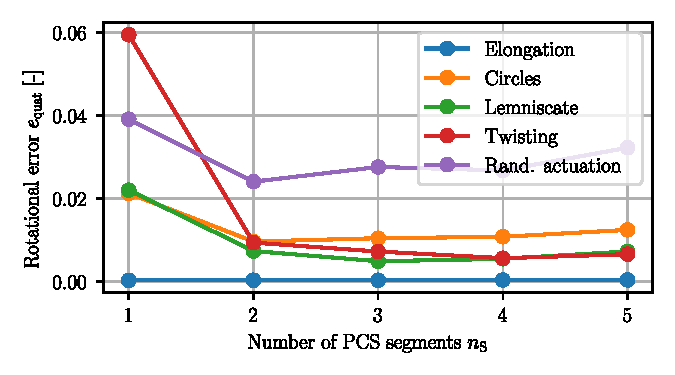
\includegraphics[width=0.49\columnwidth]{hsamodel/figures/simulation_plots/Kinematic_rotation_error_vs._number_of_PCS_segments_v3_cropped.pdf}}
    
    \caption{Verification of kinematic models in simulation. 
    The plot in the first row shows the positional error $e_\mathrm{p}$ of the kinematic model against the simulated HSA. The plot in the second row visualizes the rotational error metric $e_\mathrm{quat}$, which is based on the vector component of the unit quaternion. For more information on the evaluation metrics, we refer to Section~\ref{ssub:hsamodel:hsa_rod_kinematics:evaluation_metrics}.
    %The poses of $25$ points along the rod determined through forward kinematics of a regressed configuration are compared against the links of a simulated, discretized Cosserat rod. 
    The kinematic model used here assumes the twist \& stretch strains to be constant along the entire HSA and the bend \& shear strains to be captured by $n_\mathrm{S}$ segments.
    Along this line, we report the performance of the kinematic model for a parametrization containing one to five segments.
    }\label{fig:hsamodel:hsa_robot_simulation_kinematic_error_vs_number_of_PCS_segments}
\end{figure}

% \subsection{Differential Kinematics}
% Derive Jacobian etc.

% \begin{SCfigure*}
%     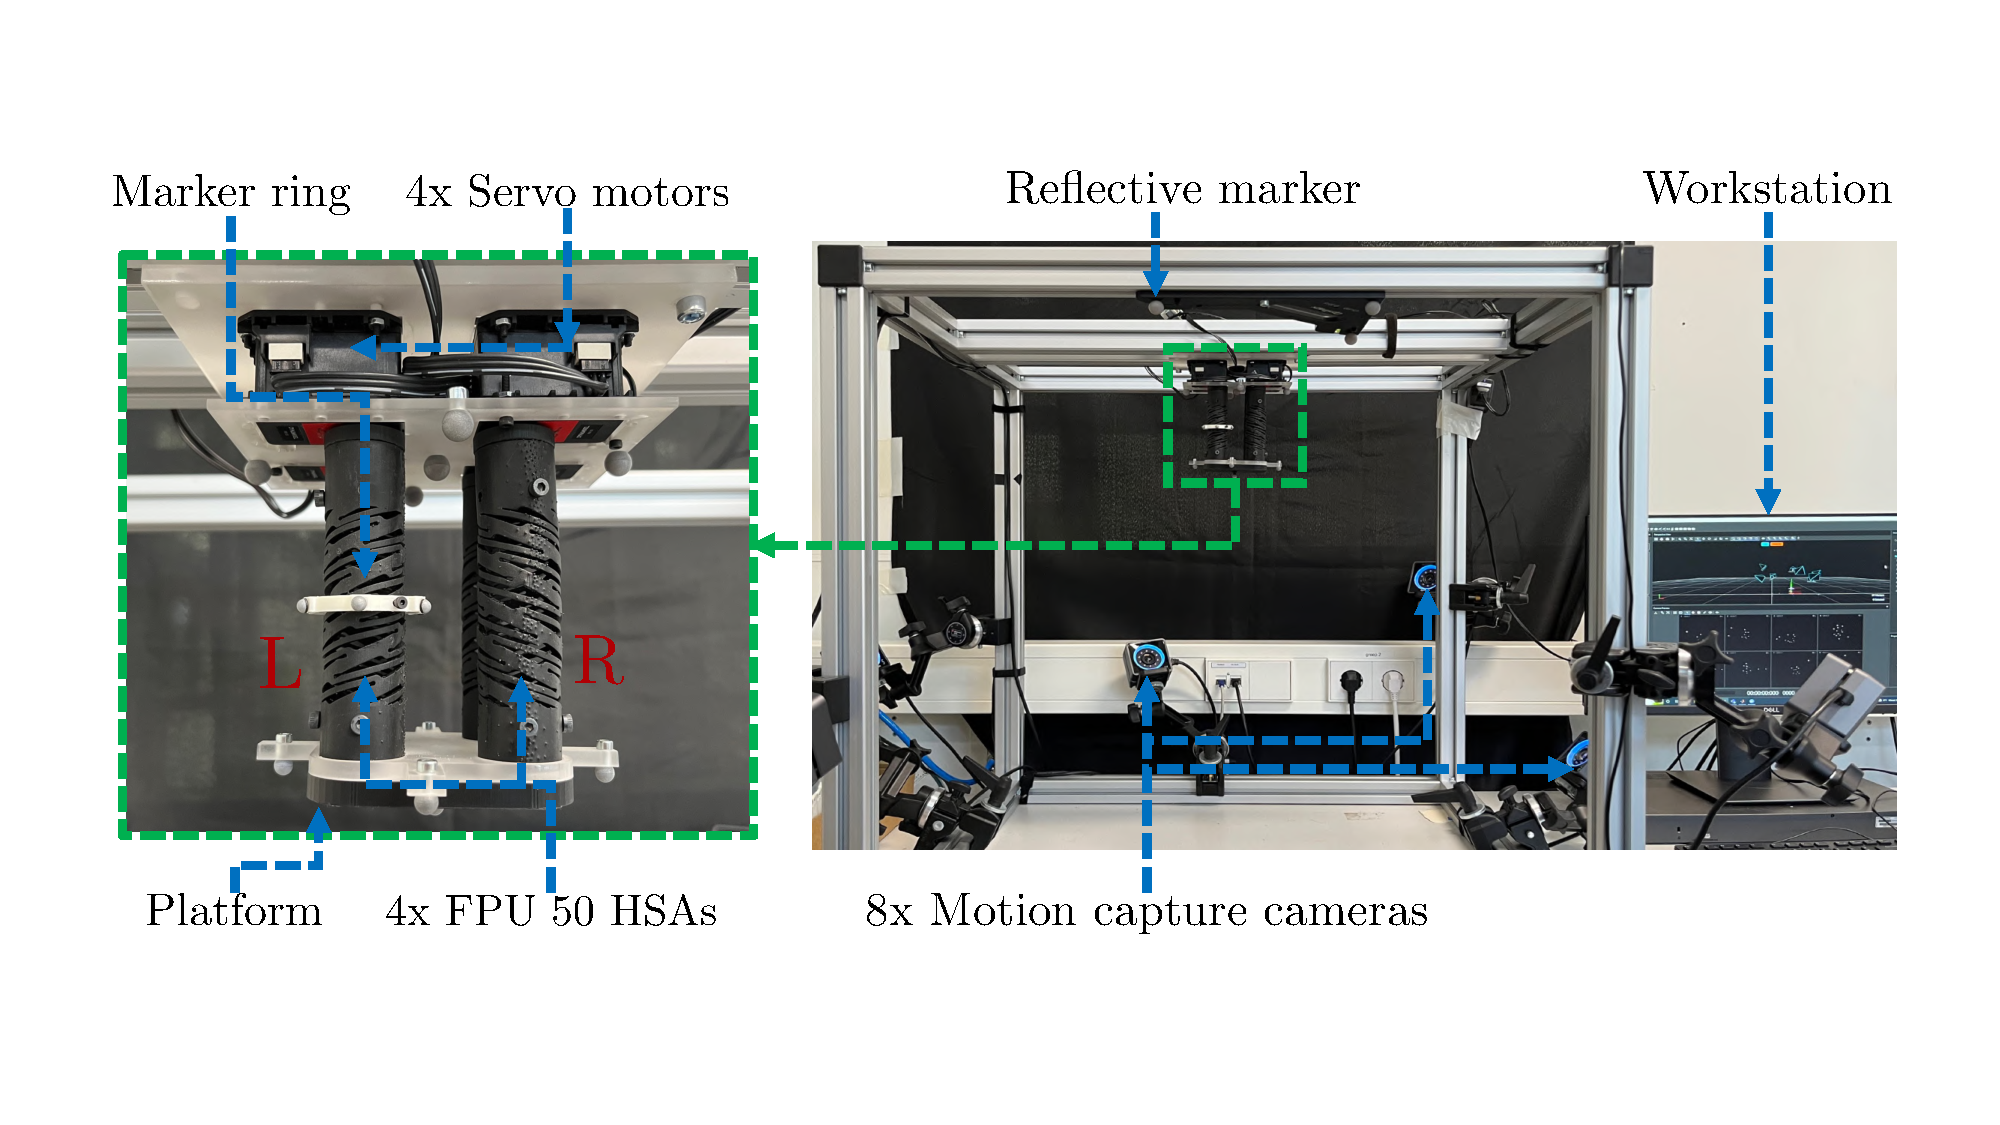
\includegraphics[width=0.75\textwidth]{hsamodel/figures/experimental_setup/experimental_setup_v3_compressed.pdf}
%     \caption{Experimental setup with the \gls{HSA} robot attached in platform-down configuration to the motion capture cage. The robot contains two left-handed (L) and two right-handed (R) \gls{HSA} rods respectively. Rods of the same handedness are placed opposite of each other. The reflective markers allow us to determine the pose information of the base, an intermediate point along the left \gls{HSA} rod, and the platform.}\label{fig:hsamodel:experimental_setup}
% \end{SCfigure*}

\begin{figure*}
    \centering
    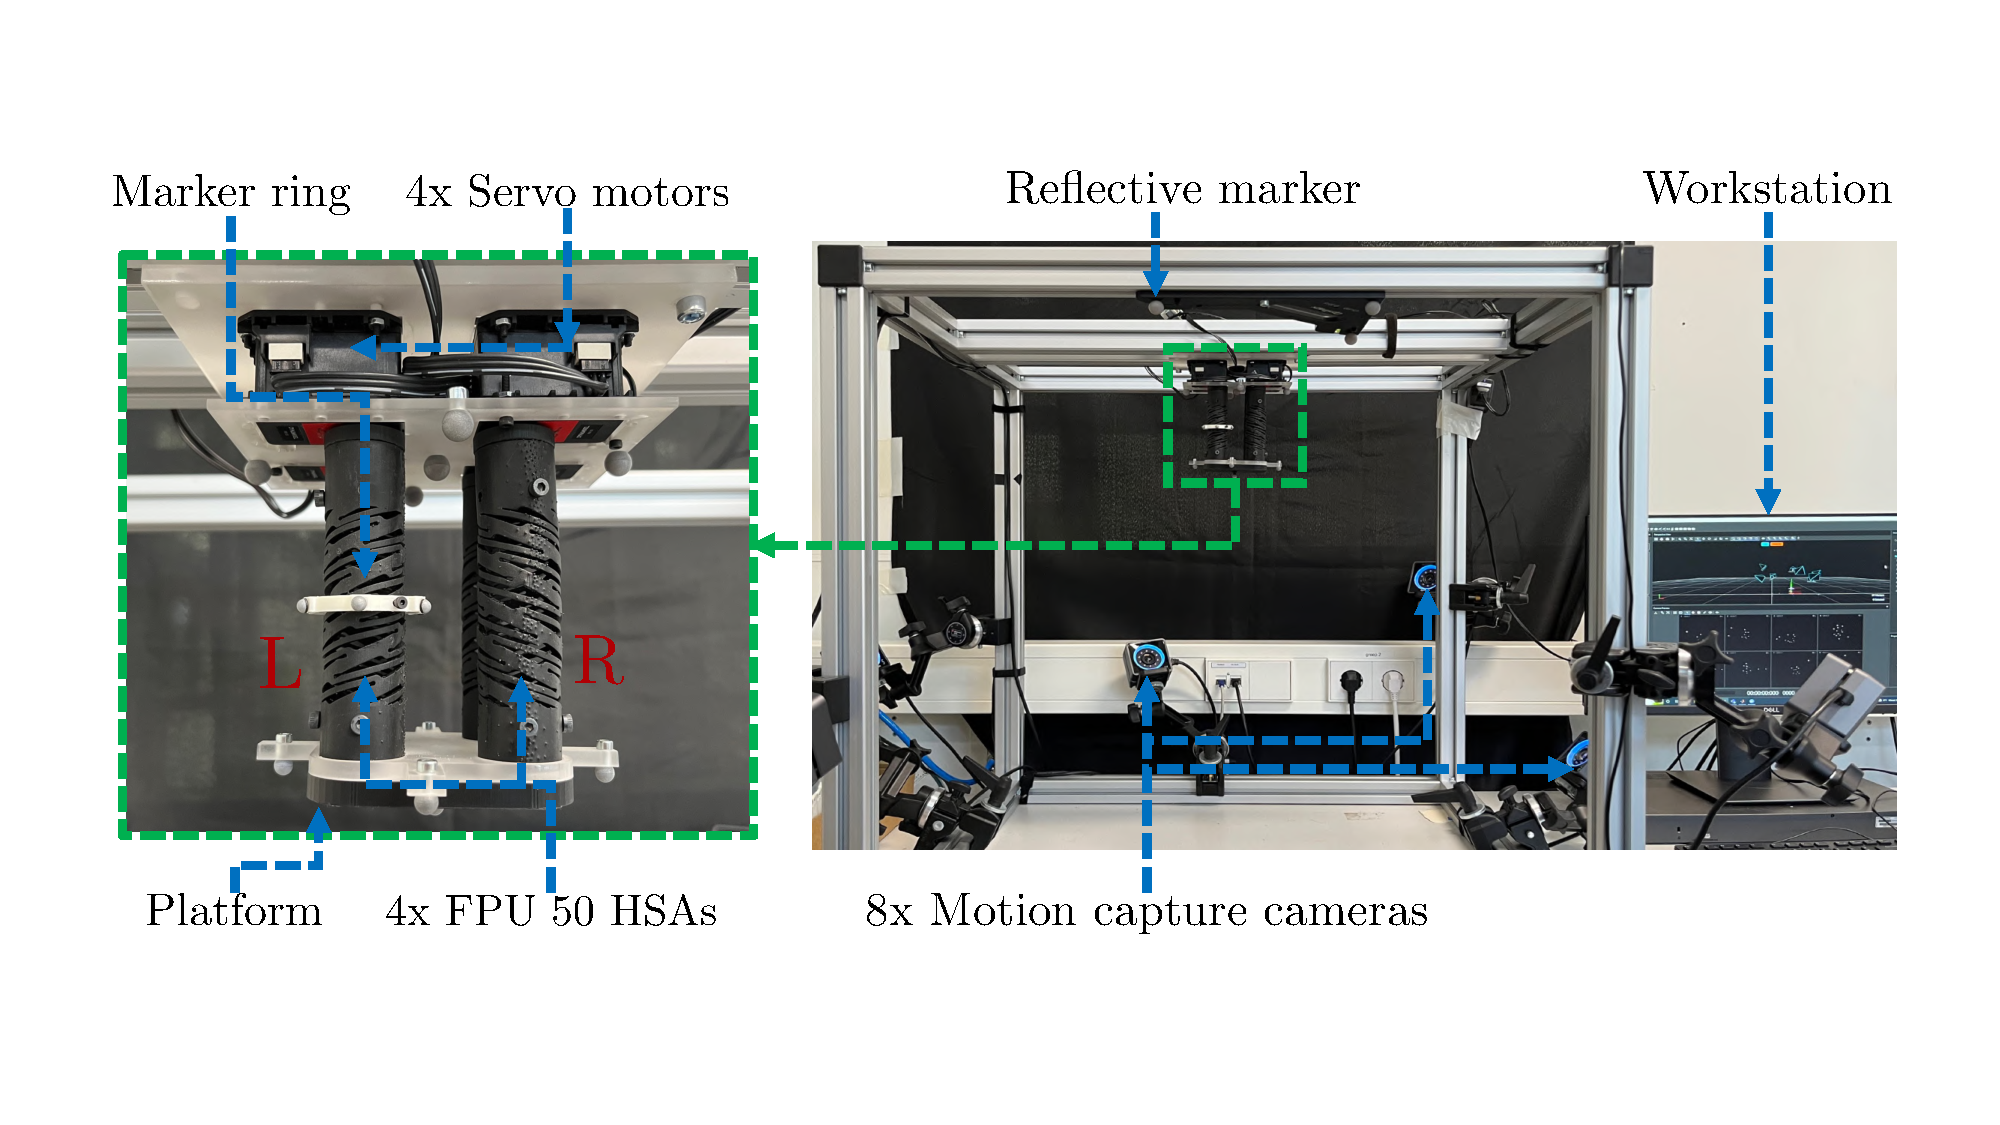
\includegraphics[width=0.77\textwidth]{hsamodel/figures/experimental_setup/experimental_setup_v3_compressed.pdf}
    \caption{Experimental setup with the \gls{HSA} robot attached in platform-down configuration to the motion capture cage. The robot contains two left-handed (L) and two right-handed (R) \gls{HSA} rods, respectively. Rods of the same handedness are placed opposite of each other. The reflective markers allow us to determine the pose information of the base, an intermediate point along the left \gls{HSA} rod, and the platform.}\label{fig:hsamodel:experimental_setup}
\end{figure*}



\subsection{Verification of SPCS Kinematics}\label{sub:hsamodel:hsa_rod_kinematics:verification}
The section is structured as follows. We introduce relevant actuation sequences for the \gls{HSA} robot.
Next, we present an inverse kinematic approach to identify the kinematic configuration.
Translational and rotational error metrics are then defined to evaluate the quality of reconstructions. %mismatch between the poses predicted by the kinematic model and the actual measurements.
% Finally, we investigate the importance of the various strains and the performance with respect to the number of \gls{CS} segments for both simulation data and experimental datasets.
Finally, we verify the performance of the proposed \gls{SPCS} kinematic model both for simulated data and on experimental datasets.
The code and all datasets are made available on GitHub~\footnote{\url{https://github.com/tud-phi/hsa-kinematic-model}}.

\subsubsection{Actuation Sequences}\label{ssub:hsamodel:hsa_rod_kinematics:actuation_sequences}
We collect datasets with a variety of actuation sequences, which include both pure motion primitives and random actuation. 
% The elongation, bending, and twisting motion primitives are invoked with the specifications in Fig.~\ref{fig:hsamodel:motion_primitives}(a). 
For all sequences, we apply a twist angle of magnitude  $|u_\mathrm{d}| \in [0, \pi \: \si{rad}]$ at the base of each \gls{HSA}. The sign of $u_\mathrm{d}$ is determined by the handedness $h$ of the respective \gls{HSA}.
The elongation dataset consists of samples between the rest and fully-elongated \gls{HSA} state. Please refer to Fig.~\ref{fig:hsamodel:motion_primitives}(a) for more details on how each motion primitive can be invoked.
For the bending motion primitive, we consider two separate trajectory types: a) a Lemniscate trajectory and b) a trajectory containing circles of varying bending angles. The different bending angles are achieved by varying the actuation angle from $\SI{20}{\percent}$ to \SI{100}{\percent} of its maximum magnitude. For each fixed bending angle, we collect $15$ samples along the circle, e.g. $15$ different azimuth angles.
To achieve the desired azimuth angle, we smoothly interpolate between the east, north, west, and south actuation specifications of Fig.~\ref{fig:hsamodel:motion_primitives}(a).
The twisting trajectory collects discrete samples between maximum clockwise (CW) and maximum counterclockwise (CCW) twisting.
Finally, we collect a dataset of randomly sampled actuation inputs, which combines the elongation, bending, and twisting motion primitives. % More specifically, we randomly the azimuth angle of bending from a uniform distribution $\mathcal{U}(0,2\pi)$.
In total, the elongation and Lemniscate trajectories contain $100$ samples each, and the circles and twisting trajectory have $225$ and $100$ samples, respectively. $500$ samples are included in the random actuation sequence.


% We consider different datasets as part of this study. In some datasets, we actuate the \gls{HSA} robot such as to exhibit one of the motion primitives purely (e.g. elongation, bending, and twisting). Contrarily, the \emph{random actuation} dataset combines these motion primitives as we randomly sample each motor position $u_j \in h_j \, \mathcal{U}(0,\pi \, \si{rad})$. 

\subsubsection{Inverse Kinematics}\label{ssub:hsamodel:hsa_rod_kinematics:inverse_kinematics}
Differential inverse kinematics can be used to reconstruct the rod's configuration $q$ from $N$ known poses $T_{\mathcal{B}}^{s_i} \in SE(3), i \in [1, N]$ along the rod. 
%While any of the standard Jacobian-based inverse differential kinematics approaches from literature~\citep{siciliano2009differential} could be used, 
We implemented an inverse kinematics algorithm based on the analytical Jacobian $J_\mathrm{A}^{s_i} \in \mathbb{R}^{6 \times 7}$ of the pose representation
\begin{equation*}
    \chi_{\mathcal{B}}^{s_i} = \begin{pmatrix}
        \varepsilon_x & \varepsilon_y & \varepsilon_z & \eta & \varepsilon_z & p_x & p_y & p_z
    \end{pmatrix}^\top \in \mathbb{R}^{7},
\end{equation*}
which includes rotational orientation estimates in unit quaternion representation $\mathcal{Q} = \begin{pmatrix} \varepsilon_x & \varepsilon_y & \varepsilon_z & \eta \end{pmatrix}^\top$ and positions in Cartesian space $p = \begin{pmatrix} p_x & p_y & p_z \end{pmatrix}^\top$.
Please note that usually $\phi_0$ does not need to be found through (differential) inverse kinematics but can rather be directly read out from the encoders of the electric servos.
All $N$ poses and Jacobians can be vertically stacked as $\chi \in \mathbb{R}^{7N}$  and $J_\mathrm{A} \in \mathbb{R}^{7N \times 6}$  respectively. This then allows us to iteratively optimize the pose error $e_\chi = \chi_\mathrm{d} - \tilde{\chi}$ between the known pose $\chi_\mathrm{d}$ and the pose $\tilde{\chi}$ computed using the forward kinematics
\begin{equation}
    \tilde{q}_{\mathrm{it} + 1} = \tilde{q}_{\mathrm{it}} + \lambda \, J_\mathrm{A}^\top(\tilde{q}) \, \left ( \chi_\mathrm{d} - \tilde{\chi}(\tilde{q}) \right ),
\end{equation}
where $\tilde{q}$ is the current configuration estimate, and $\lambda$ is the step size.

\begingroup
\setlength{\tabcolsep}{2pt} % Default value: 6pt
\begin{table}\scriptsize
\centering
\caption{Experimental verification of kinematic models on an HSA robot. Motion capture markers attached to one of the \glspl{HSA} provide two ground-truth poses along the rod,
and we measure $\phi_0$ from the servo readings ($13$ constraints in total). %Therefore, we have in total $13$ constrains for the kinematic model.
% We evaluate on a variety of datasets collected with actuation sequences mirroring certain motion primitives such as pure elongation, pure bending, and pure twisting. Additionally, we also consider a dataset with random actuation angles. As a consequence, this dataset contains samples exhibiting all three motion primitives simultaneously. 
In the spirit of an ablation study, we investigate different variations of the proposed kinematic parametrization.
For Constant Curvature (CC), Constant Twist (CT), Constant Shear (CSH), and Constant Axial (CA) strain, the strain is kept constant along the entire HSA.
For Piecewise Constant Curvature (PCC), Piecewise Constant Twist (PCT), Piecewise Constant Shear (PCSH), and Piecewise Constant Axial (PCA) strain, the strain components are parameterized separately for each of the two segments.
% All kinematic parametrization use two Piecewise Constant Strain (PCS) segments.
Additionally, we test the importance of including the shear strain component.
For each kinematic parametrization, we state the \glspl{DOF}. 
We report RMSEs for both translations and rotations (see Sec.~\ref{ssub:hsamodel:hsa_rod_kinematics:evaluation_metrics}).}
\begin{tabular}{l cccc cccc c c c ccc}\toprule
\textbf{Trajectory} & \textbf{CC} & \textbf{CT} & \textbf{CSH} & \textbf{CA} & \textbf{PCC} & \textbf{PCT} & \textbf{PCSH} & \textbf{PCA} & \textbf{DOF} & $e_\mathrm{p}$ [mm] & $e_\mathrm{quat}$ [-] & $e_\mathrm{eul,\alpha}$ [rad] & $e_\mathrm{eul,\beta}$ [rad] & $e_\mathrm{eul,\gamma}$ [rad]\\
\midrule
Elongation & \xmark & \cmark & \xmark & \cmark & \cmark & \xmark & \xmark & \xmark & $7$ & $1.010$ & $0.0092$ & $0.0029$ & $0.0079$ & $0.0166$\\
Elongation & \xmark & \cmark & \xmark & \cmark & \cmark & \xmark & \cmark & \xmark & $11$ & $0.126$ & $0.0082$ & $0.0020$ & $0.0031$ & $0.0166$\\
Elongation & \xmark & \xmark & \xmark & \xmark & \cmark & \cmark & \cmark & \cmark & $13$ & $0.009$ & $0.0042$ & $0.0020$ & $0.0031$ & $0.0070$\\
\midrule
Circles & \xmark & \cmark & \xmark & \cmark & \cmark & \xmark & \xmark & \xmark & $7$ & $1.744$ & $0.0136$ & $0.0108$ & $0.0123$ & $0.0228$\\
Circles & \xmark & \cmark & \xmark & \cmark & \cmark & \xmark & \cmark & \xmark & $11$ & $0.227$ & $0.0082$ & $0.0110$ & $0.0122$ & $0.0227$\\
Circles & \xmark & \xmark & \xmark & \xmark & \cmark & \cmark & \cmark & \cmark & $13$ & $0.092$ & $0.0093$ & $0.0116$ & $0.0125$ & $0.0075$\\
\midrule
Lemniscate & \xmark & \cmark & \xmark & \cmark & \cmark & \xmark & \xmark & \xmark & $7$ & $1.227$ & $0.0098$ & $0.0042$ & $0.0051$ & $0.0195$\\
Lemniscate & \xmark & \cmark & \xmark & \cmark & \cmark & \xmark & \cmark & \xmark & $11$ & $0.215$ & $0.0082$ & $0.0045$ & $0.0053$ & $0.0195$\\
Lemniscate & \xmark & \xmark & \xmark & \xmark & \cmark & \cmark & \cmark & \cmark & $13$ & $0.023$ & $0.0052$ & $0.0043$ & $0.0054$ & $0.0076$\\
\midrule
Twisting & \xmark & \cmark & \xmark & \cmark & \cmark & \xmark & \xmark & \xmark & $7$ & $2.931$ & $0.0136$ & $0.0121$ & $0.0186$ & $0.0195$\\
Twisting & \xmark & \cmark & \xmark & \cmark & \cmark & \xmark & \cmark & \xmark & $11$ & $0.263$ & $0.0141$ & $0.0130$ & $0.0196$ & $0.0194$\\
Twisting & \xmark & \xmark & \xmark & \xmark & \cmark & \cmark & \cmark & \cmark & $13$ & $0.030$ & $0.0127$ & $0.0131$ & $0.0217$ & $0.0017$\\
\midrule
Rand. actuation & \xmark & \cmark & \xmark & \cmark & \cmark & \xmark & \xmark & \xmark & $7$ & $4.345$ & $0.0381$ & $0.0678$ & $0.0544$ & $0.0195$\\
Rand. actuation & \xmark & \cmark & \xmark & \cmark & \cmark & \xmark & \cmark & \xmark & $11$ & $0.365$ & $0.0383$ & $0.0681$ & $0.0544$ & $0.0193$\\
Rand. actuation & \xmark & \xmark & \xmark & \xmark & \cmark & \cmark & \cmark & \cmark & $13$ & $0.255$ & $0.0380$ & $0.0700$ & $0.0527$ & $0.0200$\\
\bottomrule
\end{tabular}
\label{tab:hsamodel:kinematic_results_experiments}
\end{table}
\endgroup

\begin{figure*}[t]
    \centering
    \subfigure[Lemniscate trajectory]{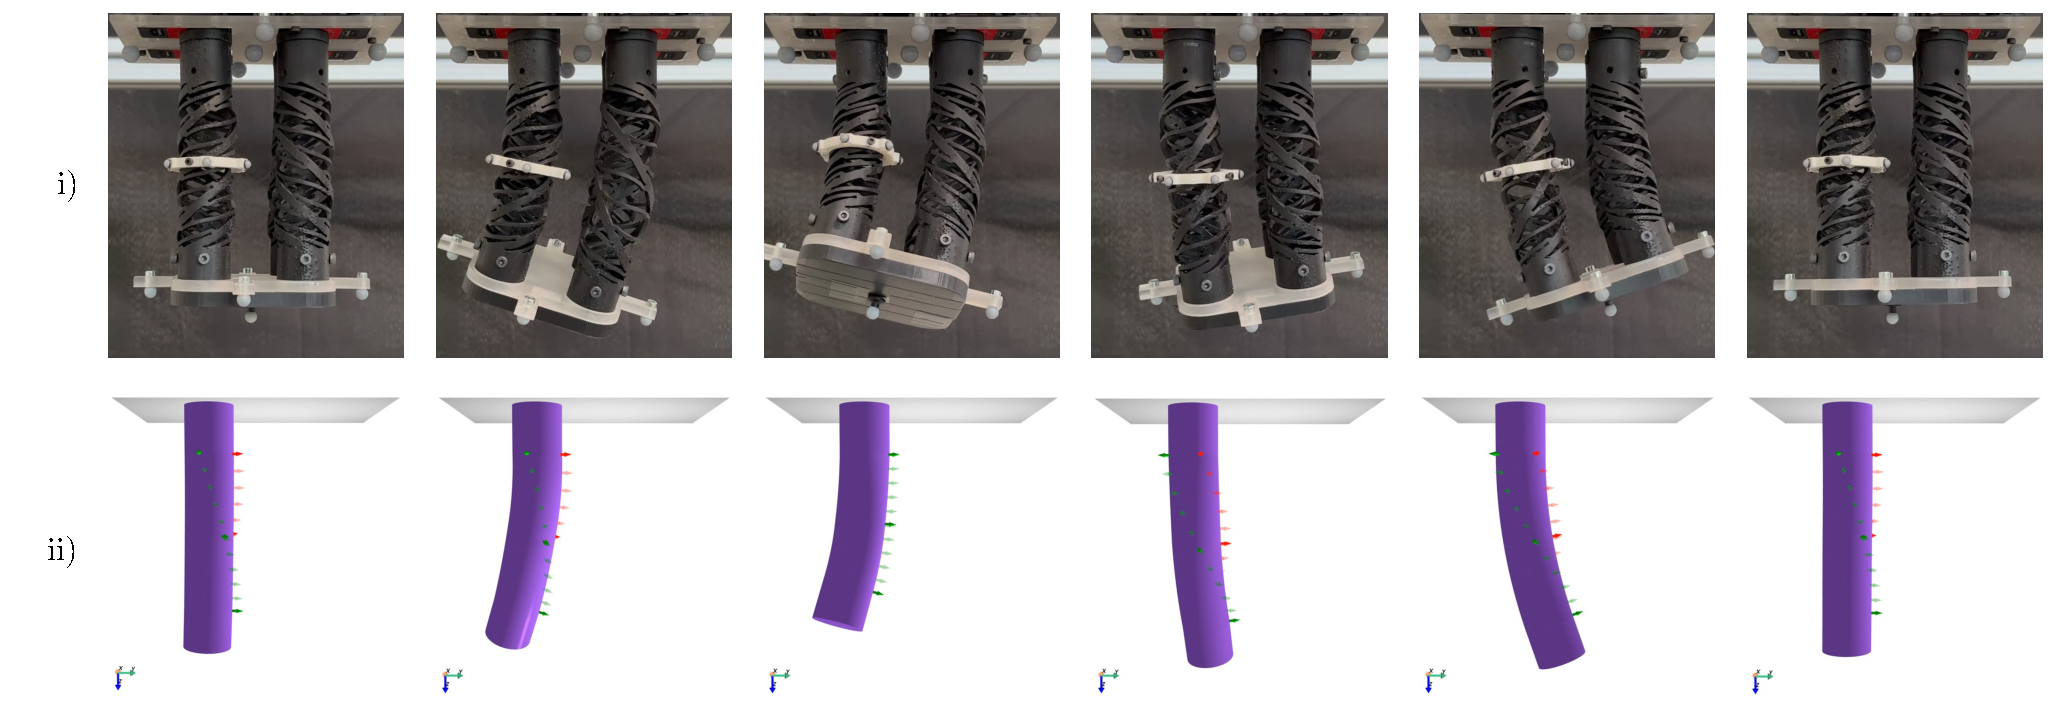
\includegraphics[width=0.95\textwidth]{hsamodel/figures/experiments_sequence_of_stills/experiment_lemniscate_inverse_kinematics_sequence_of_stills_v2_compressed.pdf}\label{fig:hsamodel:experiment_lemniscate_inverse_kinematics_sequence_of_stills}}
    \subfigure[Twisting trajectory]{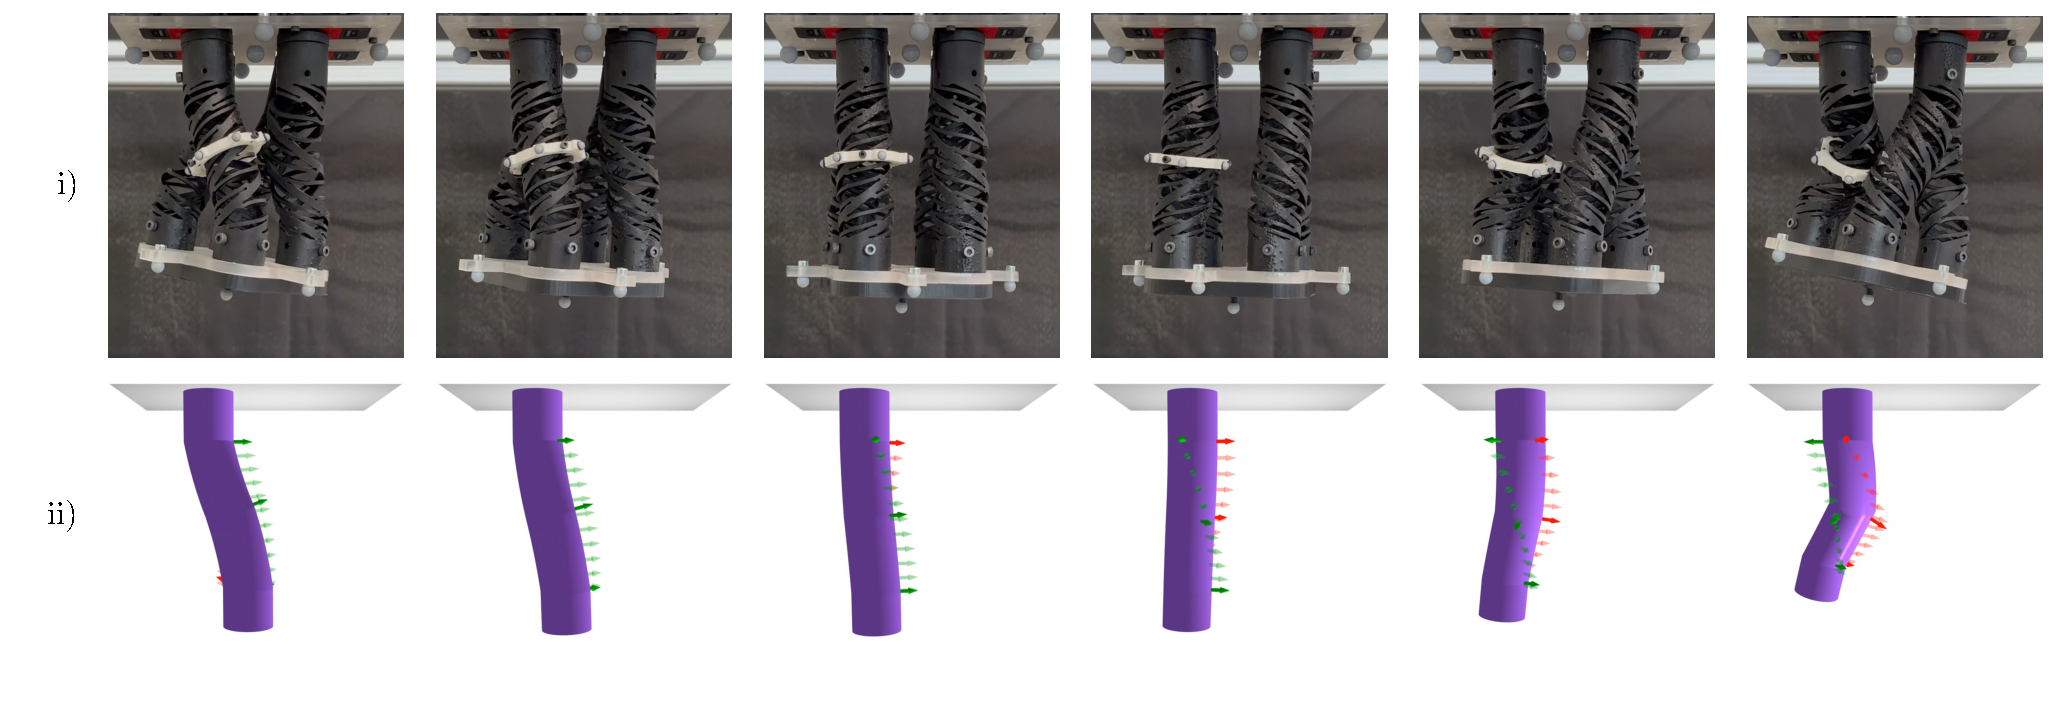
\includegraphics[width=0.9\textwidth]{hsamodel/figures/experiments_sequence_of_stills/experiment_twisting_inverse_kinematics_sequence_of_stills_v2_compressed.pdf}\label{fig:hsamodel:experiment_twisting_inverse_kinematics_sequence_of_stills}}
    
    \caption{Sequence of stills for a Lemniscate and a twisting trajectory. 
    % The numbers at the bottom signify the sample indices of the frames.
    \textbf{Top row i):} frames of a video recording of the HSA robot during the experiments. The shape of the front-left HSA rod is fitted using inverse kinematics and rendered in ii).
    \textbf{Bottom row ii):} Rendered shape of the HSA rod produced by evaluating the forward kinematics along the backbone length. The arrows with full opacity denote the ground-truth pose of three points along the HSA rod as measured by the motion capture system. The red arrow points along the local x-axis, and the green arrow along the local y-axis, respectively. The arrows with slight transparency represent poses along the backbone computed with the forward kinematics.
    We assume the last \SI{25}{mm} and \SI{20}{mm} at the proximal and distal end of the rod, respectively, to be rigid and therefore do not include them in the kinematic parametrization.
    % The white ring with the reflective motion capture markers points out the HSA rod (e.g., front-left), of which its shape is rendered in i).
    }\label{fig:hsamodel:experiment_inverse_kinematics_sequence_of_stills}
\end{figure*}

\subsubsection{Evaluation Metrics}\label{ssub:hsamodel:hsa_rod_kinematics:evaluation_metrics}
We briefly introduce the metrics to quantify shape reconstruction accuracy by the proposed kinematic parametrization. 
We first define a \gls{RMSE} for comparing each ground-truth position $p_t^i \in \mathbb{R}^{3}, t \in \{1,\dots,n_t\}, i \in \{1,\dots,N\}$ to the position estimated by the kinematic model $\tilde{p}_t^i$ over a time period of $n_t$ steps
\begin{equation}\label{eq:hsamodel:translational_rmse}
    e_{\mathrm{p}} = \sqrt{\sum_{t = 1}^{n_\mathrm{t}} \sum_{i = 1}^{N} \frac{\left (\big\lVert \tilde{p}_t^i - p_t^i \big\rVert_2 \right )^2}{n_\mathrm{t} \, N}}  \in \mathbb{R}.
\end{equation}
% Next, we compute a rotational \gls{RMSE} in unit quaternion representation
% \begin{equation}
%     e_{\mathrm{quat}} = \sqrt{\sum_{t = 1}^{n_\mathrm{t}}  \sum_{i = 1}^{N} \frac{\left (\big\lVert \tilde{\varepsilon}_t^i - \varepsilon_t^i \big\rVert_2 \right )^2}{n_\mathrm{t} \, N}} \in \mathbb{R},
% \end{equation}
% where we use the Euclidean norm of the quaternion vector component $\varepsilon = \begin{pmatrix}\varepsilon_x & \varepsilon_y & \varepsilon_z \end{pmatrix}^\top$.
The rotational \glspl{RMSE} $e_{\mathrm{quat}}$ is computed analogue by substituting $p$ in \eqref{eq:hsamodel:translational_rmse} with the quaternion vector component $\varepsilon = \begin{pmatrix}\varepsilon_x & \varepsilon_y & \varepsilon_z \end{pmatrix}^\top$.
% Finally, we compute the relative rotation between $\tilde{R} \in \mathbb{3 \times 3}$ and $R \in \mathbb{3 \times 3}$ with $e_R = R \tilde{R}^\top$. 
Finally, we compute the XYZ Euler angle error as 
\begin{equation}
    e_\mathrm{eul} = \sqrt{\sum_{t = 1}^{n_\mathrm{t}} \sum_{i = 1}^{N} \frac{\left ( f_\vartheta(R_{t,i} \, \tilde{R}_{t,i}^\top) \right )^2}{n_\mathrm{t} \, N}} \in \mathbb{R}^3,
\end{equation}
where $f_\vartheta(\cdot)$ is the operator to compute the XYZ Euler angles $\vartheta = \begin{pmatrix}\alpha & \beta & \gamma \end{pmatrix}^\top$ from a rotation matrix $R \in SO(3)$.

% Relative rotation:
% \begin{equation}
%     R_T^{\tilde{T}} = R_s^\mathcal{B} \, \tilde{R}_{\mathcal{B}}^s
% \end{equation}

\subsubsection{Simulation Results}\label{ssub:hsamodel:hsa_rod_kinematics:simulation_results}
%The suitability of the proposed, low-dimensional kinematic parametrization is first tested in simulation. 
%
We employ the higher-dimensional \gls{HSA} robot simulator proposed in Section~\ref{sec:hsamodel:hsa_robot_simulation} to generate steady-state \gls{HSA} states. We use the same simulation parameters as in Section~\ref{sub:hsamodel:hsa_robot_simulation:motion_primitives}. This provides us with $25$ discrete poses along each of the four \glspl{HSA}.
Then, we perform differential inverse kinematics with a step size of $\lambda = 0.2$ to find an optimal configuration $q$ describing the shape of the \gls{HSA}. We choose a higher step size ($\lambda=1$) for regressing the twist strains.

For the kinematic model, we assume that the twist \& stretch strains are constant along the entire \gls{HSA} rod. The bend \& shear strains, on the other hand, are instead piece-wise constant across $n_\mathrm{S}$ segments. We evaluate the influence of the $n_\mathrm{S}$ parameter and test the performance of a kinematic model involving between $1$ and $5$ \gls{PCS} segments.

The results are in Fig.~\ref{fig:hsamodel:hsa_robot_simulation_kinematic_error_vs_number_of_PCS_segments}. While a kinematic model with a single \gls{CS} segment still works sufficiently well for the elongation and bending motion primitives, its performance deteriorates for any trajectories involving twisting. Instead, two segments of our model are sufficient to accurately represent the shape of the \gls{HSA}. 

% We perform an ablation study to identify which components of the kinematic parametrization are essential for accurately representing the shape of an \gls{HSA} rod. The results in Table~\ref{tab:hsamodel:kinematic_results_simulations} show that a parametrization neglecting the shear strains is not able to model the bending or twisting motion primitives. While one \gls{CS} segment is sufficient to represent the elongation and bending motion primitives, the performance sharply deteriorates on the twisting dataset. Finally, we conclude that considering the twist strain is not necessary and does not positively influence the performance significantly. 

% \begin{figure*}[hbt]
%     \centering
%     \subfigure[Positions]{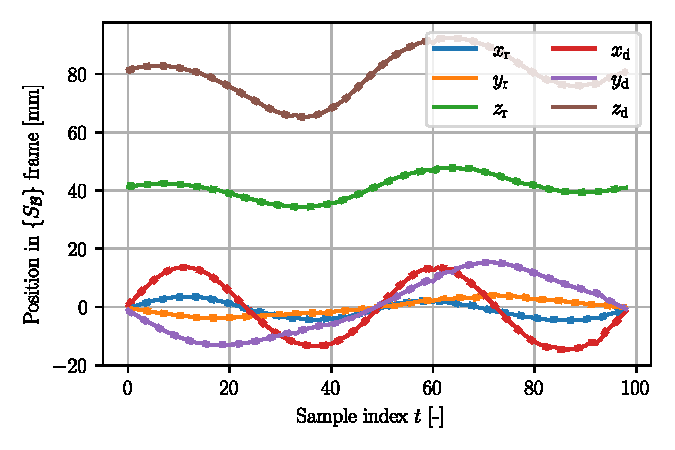
\includegraphics[width=0.49\textwidth]{hsamodel/figures/experiment_plots/inverse_kinematics_experimental_lemniscate_trajectory_positions_v4_cropped.pdf}\label{fig:hsamodel:inverse_kinematics_experimental_lemniscate_trajectory_positions}}
%     \subfigure[Euler XYZ angles]{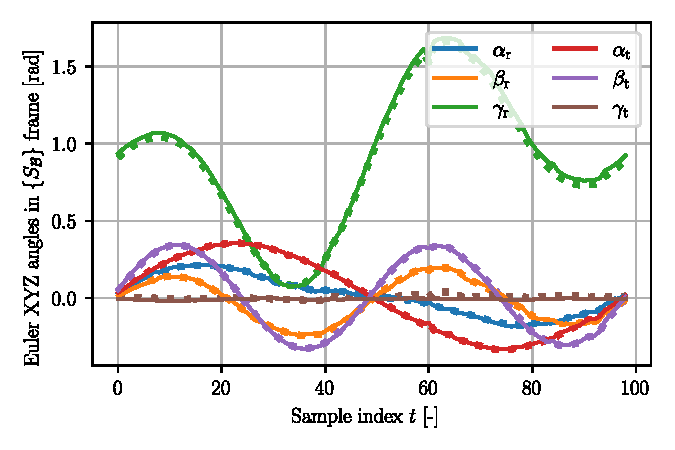
\includegraphics[width=0.49\textwidth]{hsamodel/figures/experiment_plots/inverse_kinematics_experimental_lemniscate_trajectory_euler_angles_v4_cropped.pdf}\label{fig:hsamodel:inverse_kinematics_experimental_lemniscate_trajectory_euler_angles}}
    
%     \caption{Kinematic model fitted on the experimental data of the Lemniscate actuation sequence. The solid lines denote the ground-truth poses with respect to the base frame $\{ S_{\mathcal{B}} \}$ collected by the motion capture system. The dotted lines represent the poses found when evaluating the kinematic model for the configuration $q$. This configuration was previously fitted through the means of differential inverse kinematics. The subscript $\mathrm{r}$ denotes the pose of the marker ring and the subscript $\mathrm{d}$ is connected to the pose of the distal end of the HSA rod. The kinematic model used to produce this results consists of two PCS~\citep{renda2018discrete} segments with the twist strains being neglected.}
% \end{figure*}

\subsubsection{Experimental Results}\label{ssub:hsamodel:hsa_rod_kinematics:experimental_results}
In addition to the simulations, we also experimentally verify the kinematic model using an \gls{HSA} robot consisting of four closed rods 3D-printed via digital projection lithography from the flexible photopolymer resin Carbon FPU 50~\citep{truby2021recipe}. Each \gls{HSA} rod was printed to a length of $\bar{L} = \SI{101.6}{mm}$ and is independently actuated by DYNAMIXEL MX-28T servo motors.
% Right-handed and left-handed \glspl{HSA} are placed diagonally opposite each other, respectively.
As seen in Fig.~\ref{fig:hsamodel:experimental_setup}, we attach motion capture markers to several points on the robot to track the ground-truth pose information. Namely, we measure the pose of the motor base, the platform, and the midpoint of one of the right-handed \gls{HSA} rods (i.e., the front-left \gls{HSA} on the picture). Please note that we extract the rotation angle $\phi_0$ from the servo encoders directly. The robot is mounted at its base to a cubical cage of side length \SI{750}{mm} in platform-down configuration. Eight Optitrack Prime X 13 cameras are attached to the cage, tracking the reflective markers at \SI{30}{Hz}.

We actuate the robot from a workstation next to it, with the control loop running at \SI{10}{Hz}. The control loop communicates motor position setpoints $u_\mathrm{d} \in \mathbb{R}^4$ to the servos. The inner control loop of the servos then applies the appropriate torques to guide the motors toward the desired position. As soon as the motors have reached their goal position, we wait for \SI{2}{s} to reach steady-state and then read out the pose measurements.

In Fig.~\ref{fig:hsamodel:experiment_inverse_kinematics_sequence_of_stills}, we show sequences of stills for the Lemniscate and twisting trajectory. The kinematic model used here assumes a constant twist strain along the entire rod and employs two \gls{PCS} segments to capture the remaining five strains. We see that, except for extreme twisting states, e.g., the far right image in Fig.~\ref{fig:hsamodel:experiment_twisting_inverse_kinematics_sequence_of_stills}, the kinematic model is able to represent the complex \gls{HSA} shape very well.

In Tab.~\ref{tab:hsamodel:kinematic_results_experiments}, we quantitatively evaluate multiple kinematic models on the trajectories defined in \ref{ssub:hsamodel:hsa_rod_kinematics:actuation_sequences}. 
The first ($7$ \glspl{DOF}) and second ($11$ \glspl{DOF}) kinematic models are very similar as both assume constant twist and constant stretch along the entire \gls{HSA}. The other strains are contained in two \gls{PCS} segments in both cases. However, the first model exhibits much larger positional errors as it neglects shear strains, which are very important in \gls{HSA} robots but were not accounted for in the literature~\citep{garg2022kinematic}.
The third model provides the upper bound on the performance, as it has with $12$ comparatively many \glspl{DOF} and uses a piecewise formulation with two segments for all segments. 
% With two poses along the rod available in the experimental data, which results in 12 constraints, it should therefore be possible to perfectly fit this kinematic model to the provided pose information.
